\chapter{Pilvi- ja konesalipalvelut\label{konesalipalvelut}}
Palvelimien toiminta-alustana voi olla perinteinen konesalipalvelu tai pilvipalvelu. Palvelujen tarjoajilla on erilaisia ratkaisuja molempiin ympäristöihin ja palveluiden vertailu on tärkeää, jolla yritys osaa ostaa oikeanlaisen palvelun tarpeisiinsa. 

Nykyaikaiset tietotekniset järjestelmät vaativat tietokonealustan, jossa ne voivat toimia tehokkaasti. Perinteisesti yrityksien tietokoneet ovat olleet konesaleissa, joka mahdollistaa useamman tietokoneet sijoittamisen kustannustehokkaasti samaan tilaan. Näitä tietokoneita, jotka palvelevat erilaisiin tietoteknisiin tarkoituksiin kutsutaan palvelimiksi \citep{server_computing}. Konesaleja vastaavasti kutsutaan palvelinsaleiksi. Alkuun palvelimet sijaitsivat yrityksen omissa tiloissa ja olivat käytössä vain yrityksen omiin tarpeisiin. Omat konesalit olivat kuitenkin kalliita rakentaa ja palvelimien ylläpito itsenäisesti oli kallista. Näin siirryttiin keskitettyihin konesaleihin, joissa yhden rakennuksen sisällä oli useamman yrityksen palvelimia. Samalla saatiin kustannuksia alemmaksi, kun ylläpitohenkilöt olivat käytettävissä useammalle yritykselle \citep{server_room}.

Seuraava kehitysaskel oli siirtyä virtuaalitietokoneisiin, joissa yksi palvelin tarjosi laskentakapasiteettia useammalle yritykselle. Palvelimien kustannuksia saatiin alemmaksi jakamalla konekustannukset useammalle yritykselle. Edelleen kuitenkin nämä palvelimet sijaitsivat fyysisesti keskitettynä konesaleissa. Tiedettiin, että oman yrityksen järjestelmät toimivat tietyssä palvelimessa, mutta tarkkaan ei ollut määritelty mitä osaa laitteesta järjestelmä käytti ja kuinka paljon laskentatehoa sillä oli käytössä \citep{virtual_server}.

Viimeisin kehitysaskel on siirtyä pilvipohjaisiin palveluihin. Pilvipohjainen palvelin muistuttaa toimintaperiaatteeltaan virtuaalista palvelinta, mutta palvelimen fyysinen sijainti ei ole tiedossa \citep{cloud_computing}. Sanotaan, että palvelin on pilvessä eli sen fyysinen sijainti on jossain epämääräisesti. Pilvipohjaisissa palveluissa palvelin voi olla dedikoitu palvelin tai virtuaalipalvelin. Dedikoitu palvelin tarkoittaa, että palvelimen käytössä olevat resurssit on kokonaan osoitettu asiakkaalle \citep{dedicated_hosting}.

Konesalipalveluja siirretään nykyisin paljon pilvipalveluiksi, koska näin saavutetaan lukuisia hyötyjä. Pilvipalvelujen avulla yritys voi vähentää laitteisto-, tietokanta-, ohjelmistolisenssi- ja käyttökustannuksiaan. Palvelujen tuottamiseen tarvitaan myös vähemmän henkilöresursseja. Pilvipalvelut ovat skaalautuvia, joten käytettävissä olevien palvelimien määrää voidaan vapaasti vaihtaa eikä palvelimien määrälle ole asetettu rajoituksia. Skaalautuminen mahdollistaa tuotantoympäristön sopeuttamisen asiakkaan tarpeiden mukaisesti. Pilvipalveluntarjoajilla on datakeskuksia fyysisesti eri paikoissa ympäri maailman, mikä tekee pilvipalveluista nopeita ja luotettavia käyttää \citep{top_cloud}.

\section{Palvelukuvaukset}
Konesalipalveluissa palvelimet sijaitsevat fyysisesti palveluntarjoajan konesaleissa tai yrityksen omassa pienemmässä konesalissa. Yritys voi ostaa palveluna joko koko palvelimen tai pienen osan palvelimesta, jolloin sitä kutsutaan virtuaalipalvelimeksi. Virtuaalipalvelimissa laskentateho ja muut palvelimen kapasiteetit on jaettu useammalle yritykselle. Konesalipalvelut sisältävät fyysisen palvelimen, sähkön, jäähdytyksen, palvelimen raudan ylläpidon ja ohjelmiston ylläpidon. Lisäksi palvelimeen voidaan ostaa siihen liittyvää tallennuskapasiteettia ja tietoliikennepalveluja. Nämä palvelut voivat olla myös dedikoituja tai jaettuja resursseja. Isot tallennuskapasiteetit voivat olla useamman palvelimen käytössä samanaikaisesti. Palveluntarjoajalla on palvelukuvaukset näistä kaikista palveluista, joita se tarjoaa asiakkaillensa \citep{handbook}.

Palvelukuvauksissa on määritelty tarkkaan vastuualueet palveluntarjoajan ja asiakkaan välillä. Kuvaukset sisältävät tiedot palvelun laadusta, sen mittaamisesta ja raportoinnista asiakkaalle. Kuvauksissa on myös määritelty laatutasot erilaisille palveluille ja palvelimille \citep{handbook}. Yrityksellä voi olla bisneskriittisiä palveluita, joiden laatutason tulee olla korkea. Toisaalta osassa palvelimia laatutaso voi olla määritelty alhaisemmaksi eivätkä vaatimukset palveluntoimittajalle ole niin suuret. Jos palveluntarjoaja ei pääse palvelukuvauksessa vaadittuihin laatutasoihin, niin sopimukset määrittelevät rahalliset sanktiot.

Palvelun laadun määrittelemiseen käytetään termejä \emph{availability} eli saavutettavuus sekä \emph{reliability} eli luotettavuus. Saavutettavuus tarkoittaa, että kuinka paljon ajan funktiona palvelin on käytössä eli toiminnassa. Esimerkiksi sähkö- tai tietoliikennekatko estää palvelimen käytön. Luotettavuus ja käytettävyys termit tarkoittavat, että kuinka paljon ajan funktiona palvelimen ohjelmisto on käytössä \citep{service_availability} \citep{itil}. Tämä mittari kertoo sen, voiko asiakas käyttää ohjelmaa, joka on palvelimella. Esimerkiksi ohjelmistovirhe voi estää palvelimella suoritettavan ohjelman käytön. Toisaalta jos palvelin ei ole saavutettavissa, niin sen käytettävyys on myös nolla. Näiden termien eroavaisuus on tärkeä huomioida. Yleensä konesalipalveluissa palvelutarjoaja myy tiettyä saavutettavuutta, joka on määritelty palvelutasosopimuksessa (Service Level Agreement) SLA. Jos palvelin on toiminnassa, mutta ohjelma ei toimi, niin tämä ei välttämättä ole konesalipalvelun tarjoajan ongelma. Palveluntarjoaja ainoastaan mittaa, että palvelin on saavutettavissa. Jos ohjelmisto ostetaan (Software as a Service) SaaS palveluna, niin tällöin sopimukseen kuuluu, että ohjelmisto on käytettävissä sopimuksessa määritellyn ajan ilman katkoja \citep{software_service}. SaaS sopimuksen mukaisesti ohjelman pitää koko ajan olla käytettävissä ja toimia. SaaS palvelussa tarjoaja on vastuussa myös ohjelman laadusta, että se toimii.

\section{Palvelujen tarjoajat}
Yhden määritelmän mukaisesti konesali on tekninen tila, joka on operatiivisessa käytössä tai varalla tietoteknisille laitteille. Pieniä konesaleja kutsutaan palvelinhuoneiksi (\emph{server room}) ja suurempia datakeskuksiksi (\emph{data center}). Konesalipalveluilla tarkoitetaan liiketoimintamallia, jossa organisaatio tarjoaa konesalinsa kapasiteettia toisille yrityksille korvausta vastaan. Konesali voi olla omistettu kokonaan yhdelle toimijalle (ns. oma konesali) tai konesalin kapasiteettia voidaan tarjota useammalle toimijalle (ns. yhteiskäyttöinen tai kaupallinen konesali) \citep{itewiki}.

Pienempiä yrityksiä, jotka tarjoavat konesalipalveluja on lukuisia Suomessa. Osa niistä on erikoistunut tietylle teollisuuden alalle tai maantieteellisesti tietylle alueelle. Nämä pienemmät konesalit ovat usein syntyneet ulkoistuksen kautta. Yrityksellä on ollut oma konesali, joka on sitten ulkoistettu omaksi palveluyritykseksi. Nämä konesaliyritykset tarjoavat nykyään palveluja useammalle yritykselle \citep{tnnet}.

Pienemmät konesalit eivät ole varteen otettavia vaihtoehtoja isoille yrityksille, joilla tulee olla mahdollisuus laajentaa IT-palveluja lisäämällä kapasiteettia. Isojen yrityksien konesalit onkin ulkoistuttu isoille IT-taloille. Näitä isoja palvelujen tarjoajia on vain muutamia tällä hetkellä Suomessa. Julkisista asiakirjoista selviää näiden isojen IT-talojen nimet. Nämä isot IT-yritykset ovat vastanneet laaja-alaisiin konesalipalveluiden hankintasopimuksien tarjouspyyntöihin \citep{nurmijarvi}. Ulkomaalaisia konesalipalvelujen tarjoaja on lukuisia, mutta harvemmin fyysisiä palvelimia halutaan siirtää ulkomaille.

Pilvipalvelujen osalta palvelujen tarjoajat jakautuu kolmeen alueeseen: isot palvelujen tarjoajat, pienet palvelujen tarjoajat ja erikoistuneet palvelujen tarjoajat. Pienet palvelujen tarjoajat eivät ole varteen otettavia vaihtoehtoja, kun tarkastellaan isojen yrityksien IT-palveluja. Erikoistuneet yritykset taas tarjoavat vain tietynlaista konesalialustaa. Esimerkiksi erikoistuneesta pilvipalvelusta on Salesforce, joka tällä hetkellä maailman 7. suurin pilvipalvelujen tarjoaja. Salesforce tarjoaa vain heidän omaa alustaansa, jonka päälle tulee rakentaa omat sovellukset. Tätä mallia kutsutaan (Platform as a Service) PaaS palveluksi \citep{top_cloud}.

Tässä tutkimuksessa keskitytään isojen pilvipalvelujen tarkasteluun, koska tutkimuksen kohteena olevan Finnairin IT-palvelujen koko niin suuri, että pienet palveluyrityksen eivät ole varteen otettavia vaihtoehtoja. Kuva \ref{gartner} esittää Gartnerin nelikantamallin mukaisesti mitkä ovat johtavia pilvipalveluyrityksiä. Isoimmat pilvipalveluja tuottavat yritykset ovat: AWS, Azure ja Google Cloud.

\begin{figure}[ht]
\centering 
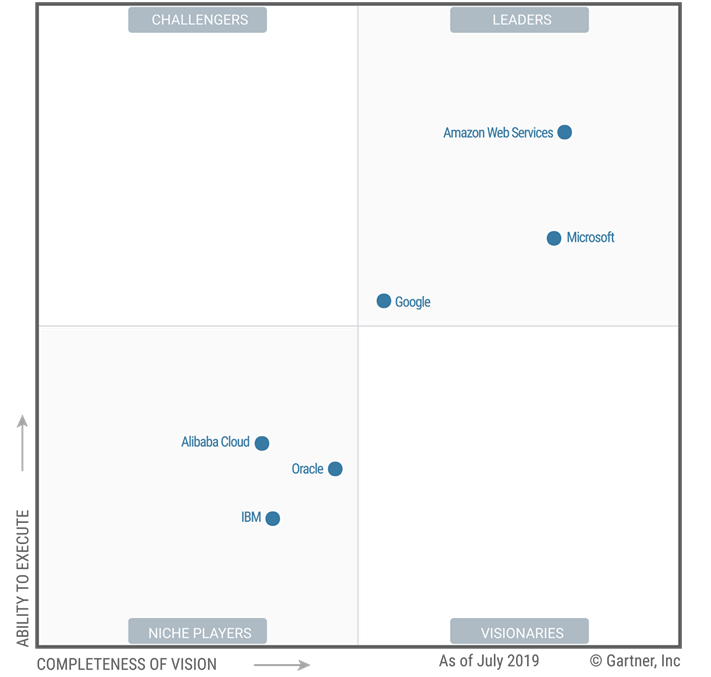
\includegraphics[width=0.50\textwidth]{figures/CloudIaaS.png}
\caption{Gartner (07/2019) pilvipalveluiden vertailu. \citep{top_cloud}}\label{gartner}
\end{figure}

Kuvassa \ref{canalys} esitetyn Canalys yrityksen raportin mukaan AWS pilvipalvelut kasvoivat 28 \% vuosien 2018–-2020 aikana. Azure pilvipalvelut kasvoivat 50 \%, Google pilvipalvelut kasvoivat 58 \% ja Alibaban pilvipalvelut kasvoivat 54 \%. Kuvasta nähdään myös, että pilvipalveluiden kysyntä on kasvanut paljon viime vuosien aikana. Viime vuosina isoimmat pilvipalveluiden tarjoajat ovat pysyneet samoina.

\begin{figure}[ht]
\centering 
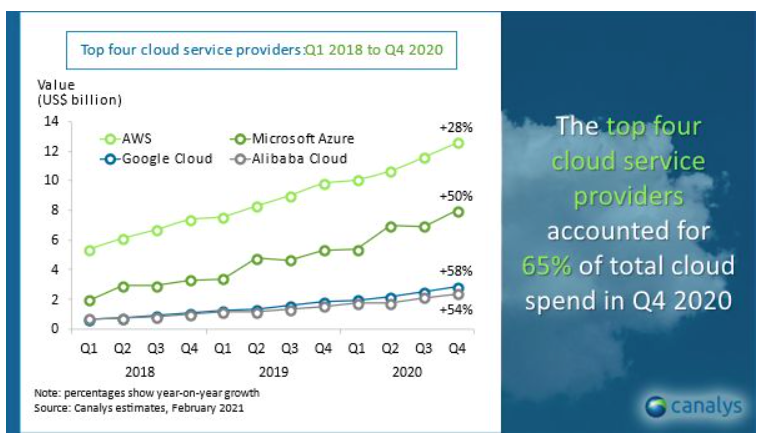
\includegraphics[width=0.70\textwidth]{figures/Canalys.png}
\caption{Canalys estimates (02/2021) pilvipalveluiden prosenttiosuudet \citep{top_cloud}}\label{canalys}
\end{figure}

(Amazon Wer Services) AWS on Amazon yhtiön pilvipalvelualusta, joka on julkaistu vuonna 2002. AWS on tällä hetkellä suosituin pilvipalvelu maailmassa ja se tarjoaa yli 165 erilaista toiminnallisuutta maailmanlaajuisesti. AWS on panostanut palveluiden turvallisuuteen ja heillä on valmiina ratkaisuja, jotka täyttävät yleisimmät tietoturvavaatimukset. AWS palvelut on sertifiointi maailmanlaajuisesti ja sertifikaatit kattavat yleisimmät ISO standardit. AWS:lla on fyysisiä konesaleja enemmän kuin millään muulla pilvipalveluiden tarjoajalla \citep{top_cloud}.

Azure on Microsoftin omistama pilvipalvelu. Azure on tällä hetkellä nopeinten kasvava pilvipalvelun tarjoaja ja Azure tavoitteena on saavuttaa kärkisija pilvipalveluiden toimittajana tulevina vuosina. Azure on viime aikoina voittanut Yhdysvalloissa isoja valtiohallinnan kilpailutuksia. Azure toiminnallisuuksien määrä ei ole niin laaja verrattuna kilpailijoihin, mutta Azuren palvelut kattavat tärkeimmät pilvipalvelun ominaisuudet. Azure pystyy tarjoamaan pilvipalveluidensa kautta Microsoftin omia tuotteita kuluttajille. Azure pilvipalvelut kattavat laajat tietoturvaominaisuudet ja maailmanlaajuiset sertifikaatit \citep{top_cloud}.

Google Cloud on Googlen omistama pilvipalvelu. Google Cloud tarjoaa vastaavia pilvipalvelun ominaisuuksia ja palveluja kuin muut pilvipalvelujen toimittajat. Google Cloud on pienempi kuin kilpailijansa AWS ja Azure. Google Cloud on erikoistunut tarjoamaan Google omia palveluitaan kuluttajille pilven kautta \citep{top_cloud}.
